\documentclass[10pt,twocolumn,letterpaper]{article}

\usepackage{cvpr}
\usepackage{times}
\usepackage{epsfig}
\usepackage{graphicx}
\usepackage{amsmath}
\usepackage{amssymb}

% Include other packages here, before hyperref.

% If you comment hyperref and then uncomment it, you should delete
% egpaper.aux before re-running latex.  (Or just hit 'q' on the first latex
% run, let it finish, and you should be clear).
\usepackage[breaklinks=true,bookmarks=false]{hyperref}

\cvprfinalcopy % *** Uncomment this line for the final submission

\def\cvprPaperID{****} % *** Enter the CVPR Paper ID here
\def\httilde{\mbox{\tt\raisebox{-.5ex}{\symbol{126}}}}

% Pages are numbered in submission mode, and unnumbered in camera-ready
%\ifcvprfinal\pagestyle{empty}\fi
\setcounter{page}{1}
\begin{document}

%%%%%%%%% TITLE
\title{An Implementation of the Classic++ Algorithm for Optical Flow}

\author{Anon. author 1
% For a paper whose authors are all at the same institution,
% omit the following lines up until the closing ``}''.
% Additional authors and addresses can be added with ``\and'',
% just like the second author.
% To save space, use either the email address or home page, not both
\and
Anon. author 2
}

\maketitle
%\thispagestyle{empty}
\begin{abstract}
Optical flow algorithms calculate the movement of objects between consecutive frames of video, by attempting to reconstruct the displacement of every pixel from frame to frame. All optical flow algorithms are built on minimizing an objective function, but there are many ways to do this minimization, and also many possible forms of the objective function. In this project, we will implement the Classic++ optical flow algorithm and analyze the performance of different forms of smoothing and regularization.
\end{abstract}

%%%%%%%%% BODY TEXT

\section{Introduction}

Optical flow can be applied to a variety of problems, for example, it allows driverless vehicles to detect the movement of pedestrians and other cars on the road. It also allows the car to estimate its own movement. Given the motion of pixels in a series of video frames, optical flow methods can interpolate pixel locations between frames, resulting in a smoother video and a sharper display when bandwidth is limited.

Optical flow is defined as the temporal change in brightness patterns of an image due to motion of an object relative to the camera. At its core, it is the problem of calculating where each pixel moves from one frame of a video to the next. \cite{fleet} However, optical flow similar to but is not the exactly the same as a motion field. For example, a rotating perfectly uniform sphere will have no optical flow, because the brightness pattern remains the same, but it does have a motion field. In contrast, if we fix the sphere and move the light source, there will be an optical flow field due to change in brightness even though the sphere does not move.

The changes in pixel intensity between frames are represented as a vector field. The motion of each pixel is represented as a flow vector $[x, y]$. The essential constraint governing the image $I$ and the flow fields $X$ and $Y$ is
\begin{equation} \label{eq:constraint}
I_x \cdot X+ I_y \cdot Y + I_t = 0
\end{equation}


In qualitative terms, the change in a pixel intensity over time ($I_t$) has to equal the difference in intensity between the original pixel and the one “upstream” from it in the flow field. Eq. \ref{eq:constraint} can also be expressed in discrete space:
\begin{equation} \label{eq:discrete}
I[x, y, t_1] = I[x + U[x, y], y + V[x, y], t_2]
\end{equation}

However, this equation results in only one constraint per pixel, whereas there are two flow vector unknowns per pixel. Therefore, this problem is underconstrained. \cite{wu} Optical flow algorithms will add additional constraints, called a penalty function, usually to represent the requirement that the optical flow of two neighboring pixels is similar. Intuitively, this is due to the fact that in natural images neighboring pixels do not move independently of each other. While almost all optical flow algorithms use Eq. \ref{eq:constraint}, different algorithms apply different penalty functions and numerical techniques to solve or optimize the resulting equations.

\section{Prior Work}
The optical flow formulation was originally proposed by Horn and Schunck (HS) \cite{horn}, who recognized that discontinuities only occur as a result of occlusion and neighboring pixels generally do not move independently. This discovery allowed them to constrain the problem by minimizing the square of the gradient of the flow vector. A flow field that changes abruptly from pixel to pixel will have a large-magnitude gradient on average, whereas a smooth flow field, such as a brightness pattern, will have a small gradient. The HS algorithm minimizes the following quantity:
\begin{multline} \label{eq:hsObj}
e = \int \int_{img} (I_x \cdot X + I_y \cdot Y + I_t)^2 + \\
\lambda ( ||\nabla X||^2 + ||\nabla Y||^2 ) dA
\end{multline}
(Throughout this document, matrix multiplication will be element-wise, not dot-product-wise, unless otherwise noted.)

The first term represents how well the flow vector field explains the pixel motion in the video, and should be 0 for a perfect flow field. The second term is the penalty function discussed above, which penalizes sudden changes in flow. The $\lambda$ parameter controls the desired smoothness of the outcome. The HS paper derived a closed form expression for the minimizing values of $X$ and $Y$, but computing power was too expensive at the time for the expression to be practical. Instead, an approximation scheme was used to iteratively converge on the minimizing values.

Since then, many modifications have been proposed to the HS minimization problem. Robust penalty terms have been developed, in which the derivatives of the flow vector are raised to a smaller power. For example, a popular penalty function, called the Charbonnier penalty function (Eq. \ref{eq:cPenalty}), is used in the Classic++ algorithm.
\begin{equation} \label{eq:cPenalty}
\sqrt{|| \nabla X ||^2 + || \nabla Y ||^2 + \epsilon}
\end{equation}
It is essentially linear in the gradients. Intuitively, penalty terms with smaller powers are more tolerant of some sudden changes in flow direction, which results in sharper edges in the flow field. Most penalty schemes do not result in an analytical expression for the minimum, thus optimization algorithms are required to solve the resulting problem.

The optimization method is another point of innovation. Sun \cite{sun} claims that the HS algorithm was limited by the approximation scheme it used. Modern computers can solve for the flow vector exactly, resulting in much better performance.

In this project we will implement the Classic++ algorithm developed by Sun et al. This approach improves upon the HS algorithm by using modern optimization methods, which results in improved flow estimation. It uses the Charbonnier penalty function (Eq. \ref{eq:cPenalty}), which results in a smoother penalty function, and spline-based bi-cubic interpolation.

\section{Solving the HS Objective Function}

To find optical flow, we need to minimize the objective function found in Eq. \ref{eq:hsObj}.  To do this, we will use the Euler-Lagrange equation, which gives us conditions for minimizing $e$.  Namely, if $e$ depends on a function $L$ and
\begin{equation} \label{eq:eulerL}
e = \int \int L(x, y, f, f_x, f_y) dxdy
\end{equation}
then $e$ is minimized when 
\begin{equation} \label{eq:eulerCondition}
\frac{\partial L}{\partial f} - \frac{\partial}{\partial x} \frac{\partial L}{\partial f_x} - \frac{\partial}{\partial y} \frac{\partial L}{\partial f_y} = 0
\end{equation}

The Euler-Lagrange equation applies directly to our problem, if we use two instances of it to constrain the flow fields $X$ and $Y$ separately.  For us, $L$ is simply the objective function $e$: 
\begin{multline} \label{eq:eulerL2}
L =  \int \int_{img} (I_x \cdot X + I_y \cdot Y + I_t)^2 + \\
\lambda ( X_x^2 + X_y^2 + Y_x^2 + Y_y^2 ) dA 
\end{multline}
To constrain $X$, we let $f=X$, so 
\begin{equation} \label{eq:eulerPlug1}
\frac{\partial L}{\partial X} = 2I_x (I_x X + I_y Y + I_t)
\end{equation}
\begin{equation} \label{eq:eulerPlug2}
\frac{\partial L}{\partial X_x} = 2 \lambda X_x
\end{equation}
\begin{equation} \label{eq:eulerPlug3}
\frac{\partial}{\partial x} \frac{\partial L}{\partial X_x} = 2 \lambda X_{xx}
\end{equation}
\begin{equation} \label{eq:eulerPlug4}
\frac{\partial L}{\partial X_y} = 2 \lambda X_y
\end{equation}
\begin{equation} \label{eq:eulerPlug5}
\frac{\partial}{\partial y} \frac{\partial L}{\partial X_y} = 2 \lambda X_{yy}
\end{equation}

And our final constraint is
\begin{equation} \label{eq:eulerPlug6}
I_x (I_x X + I_y Y + I_t) = \lambda (X_{xx} + X_{yy})
\end{equation}
This equation gives us one constraint for every pixel in the image.  We can apply the same logic with $f=Y$ to get another constraint per pixel:
\begin{equation} \label{eq:eulerPlug7}
I_y (I_x X + I_y Y + I_t) = \lambda (Y_{xx} + Y_{yy})
\end{equation}

Sometimes, these constraints are shown in block matrix form:
\begin{multline} \label{eq:eulerBlock}
\left[ \begin{array}{cc}
I_x^2 - \lambda (D_x^2 + D_y^2) & I_x I_y\\
I_x I_y & I_y^2 - \lambda (D_x^2 + D_y^2) \\
\end{array} \right]
\left[\begin{array}{c}
X \\
Y
\end{array} \right] \\
=-\left[ \begin{array}{c}
I_x I_t \\
I_y I_t
\end{array} \right]
\end{multline}
There are some subtleties hiding in this equation.  $X$ and $Y$ are vectors of length $w \times h$ - they are the flow vectors smushed into one column.  All of the image derivatives ($I_x$, etc.) in the left side matrix are diagonal matrices of width and height each $w \times h$.  They contain the image data along the diagonal, the same way $X$ and $Y$ contain the flow vector data in a column.  $D_x^2$ performs a second image derivative in the $x$ direction to the flow vector on which it is applied.  (This is an exception to our convention that matrix multiplication means pairwise product.  $D_x$ is applied like a dot product.)  Finally, the right hand side is in fact a single column of size $2wh \times 1$.  Unlike on the left hand side $I_x I_t$ and $I_y I_t$ are single-column, not diagonal.

\section{Implementing the Euler-Lagrange Solution}

We implemented a program in MATLAB that finds the flow vectors $X$ and $Y$ given two images.  We use the block matrix formulation (Eq. \ref{eq:eulerBlock}) to express the system of equations.  The image derivatives are computed and converted into diagonal sparse matrices.  We approximate $-(D_x^2 + D_y^2)$ with convolution by the kernel
\begin{equation} \label{eq:laplacian}
\left[ \begin{array}{ccc}
0 & -1 & 0 \\
-1 & 4 & -1 \\
0 & -1 & 0
\end{array} \right]
\end{equation}
, known as the Laplacian kernel.  This means that $L = -(D_x^2 + D_y^2)$ is a $(wh) \times (wh)$ sparse matrix, with approximately $5wh$ non-zero entries.  It is defined as follows:
\begin{equation} \label{eq:laplacian2}
L(a, b) = \begin{cases}
4 & \text{if } a = b \\
-1 & \text{if $a$ and $b$ are neighbors} \\
0 & \text{otherwise}
\end{cases}
\end{equation}

We calculate the image derivatives $I_x$ and $I_y$ using a 5-point filter $\frac{1}{12}[-1, 8, 0, -8, 1]$, and we used $\lambda = 0.1$.  With the terms in Eq. \ref{eq:eulerBlock} defined, solving for $X$ and $Y$ is simply a matter of matrix inversion.

In practice, we run multiple iterations of Eq. \ref{eq:eulerBlock} to find the final flow.  This is because the HS objective is only a linearized version of Eq. \ref{eq:discrete}, the true flow error.  For large flow values, it is not accurate.  After each iteration, we warp image 1 using the flow field found so far.  We then run another iteration using the warped image 1, and add the new flow to the total flow so far.

Unfortunately, there is no obvious stopping point for this algorithm.  Repeatedly minimizing the HS objective will refine the flow, making the warped image 1 look more and more like image 2.  However, this results in ``overfitting".  The ground truth flow is not in fact a perfect transformation from image 1 to image 2 - there are changes in illumination and occlusion between the two images.  Empirically, we found that running too many iterations caused the endpoint error to increase.  In our tests, we used 10 iterations, the same number used in \cite{sun}.

Our algorithm uses incremental multi-resolution optimization. It constructs an image pyramid, using gaussian filtering at each level. The optical flow is first computed for the image at the smallest level and it is is used as the initial estimate for the next-largest pyramid level, this is repeated until the largest pyramid level is reached. Multi-resoltion not only decreases the convergence time, but it increases accuracy when large moving objects of uniform brightness. Accuracy improves because at the largest pyramid level, the optical flow algorithm only detects movement of the edges of the object. However, the algorithm correctly detects the movement of the entire object when mult-resolution optimization is used, because the flow of the objects inner pixels is propogated through the pyramid levels.

Test cases in which large objects moved required more pyramid levels than those in which small objects moved, the larger the object, the more pyramid levels required to achieve the best score. Too many pyramid levels worsened the score, this is likely to due the fact that at the lowest level the object becomes too small and no noticeable movement occurs.

The results of our algorithm are shown in Figure \ref{fig:hs}.  The standard HS algorithm is predictably confused by the spinning circle in the lower left hand corner.  (Spinning objects violate the assumption that the flow has a small gradient.)  The boundaries are also somewhat blurry.  To measure the accuracy of our flow estimate, we use average endpoint error (EPE), which is the average displacement between each flow vector and its ground truth counterpart.  The EPE on this image is 0.322.

\begin{figure}

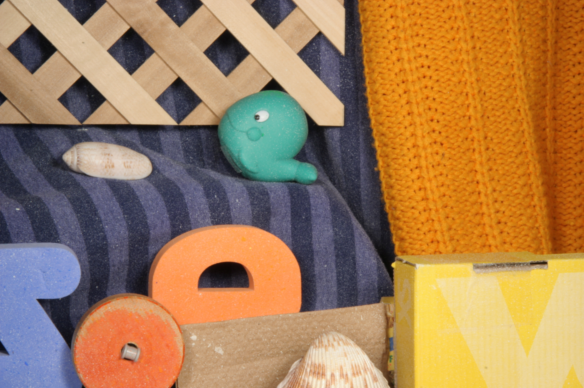
\includegraphics[width=0.6 \columnwidth] {frame10.png} 
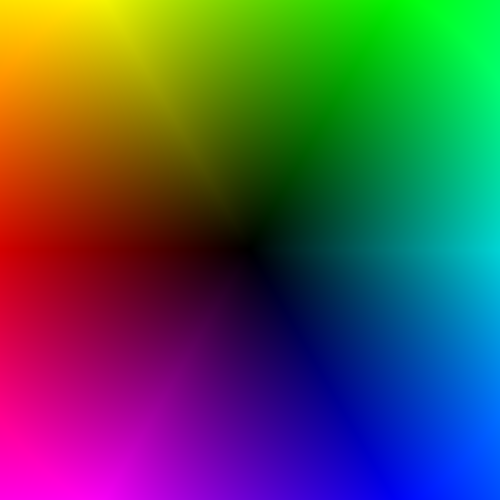
\includegraphics[width=0.39 \columnwidth] {flow-color-key.png}

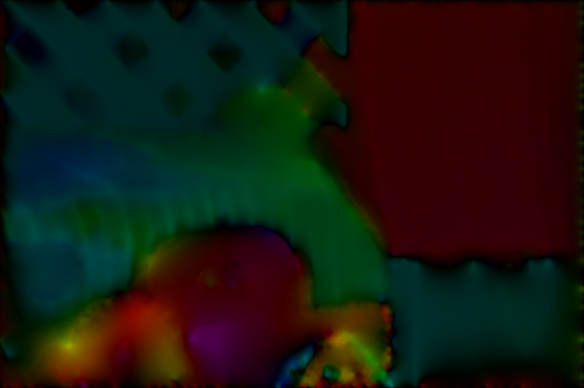
\includegraphics[width=\columnwidth]{10iter.png}

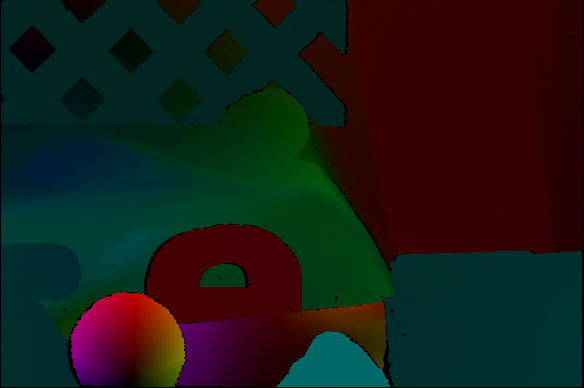
\includegraphics[width=\columnwidth]{ground_truth.png}
\caption{Top: the ``RubberWhale" test image for optical flow, and a key for the optical flow visualizations in this paper.  Middle: optical flow according to our implementation of the HS algorithm.  Bottom: ground truth flow, according to manual human labeling.}
\label{fig:hs}
\end{figure}

We test our implementation on the Middlebury optical flow benchmark \cite{middlebury}, using the 8 publicly-available training images.  The results (along with those from our improved algorithms) are shown in Figure \ref{fig:table}.

\begin{figure}

\begin{tabular} {|r | r | r|}
\hline
Image name & HS & Multi-res HS \\
\hline 
Dimetrodon & 0.5068 &  0.3832 \\
Grove2 & 1.4710 & 0.4281 \\
Grove3 &  2.4258 & 1.2280 \\
Hydrangea & 1.2445 & 0.8741 \\
RubberWhale & 0.3221 & 0.3630 \\
Urban2 & 6.9539 & 1.7945 \\
Urban3 & 5.4880 & 1.8573 \\
Venus & 1.9489 & 0.7809 \\
\hline
Average & 2.5451 & 0.9636 \\
\hline

\end{tabular}

\caption{Endpoint error by test image, for the various algorithms presented in this paper.}
\label{fig:table}
\end{figure}

From Figure \ref{fig:table}, it is obvious that our implementation of HS does not perform equally well on all test cases.  Figure \ref{fig:urban2} shows the test image with the highest error (``Urban2").  Urban2 has flow vectors with much greater magnitude, compared to RubberWhale.  The building in the foreground moves particularly quickly between frames.  The displacement is 5 pixels on average, which is further than the spatial derivatives can propagate information.  Therefore, HS cannot track the displacement of the building.  To fix this problem, we will use multi-resolution optimization later in this paper.

\begin{figure}
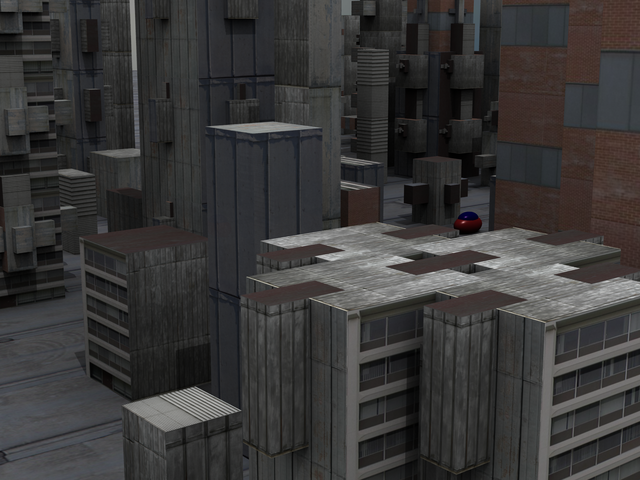
\includegraphics[width=0.48 \columnwidth] {urban2_input.png} 
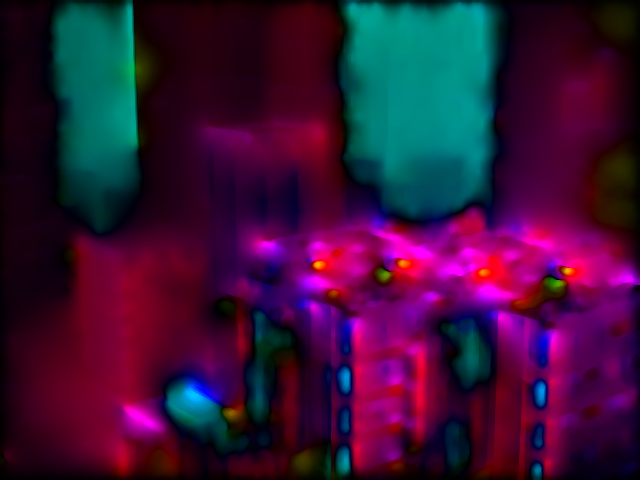
\includegraphics[width=0.48 \columnwidth] {urban2.png}

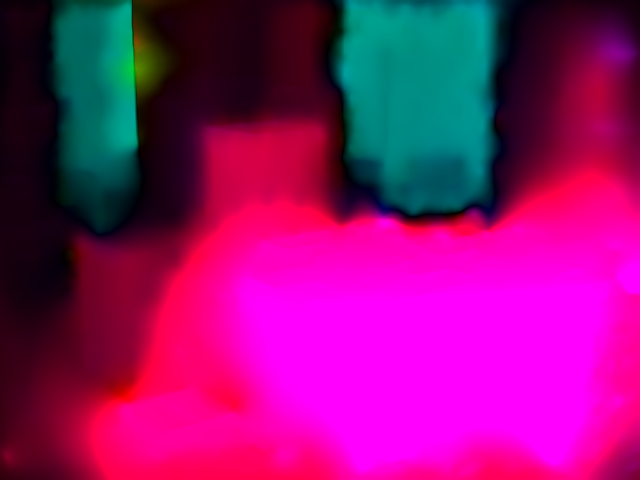
\includegraphics[width=0.48 \columnwidth] {urban2_multires.png} 
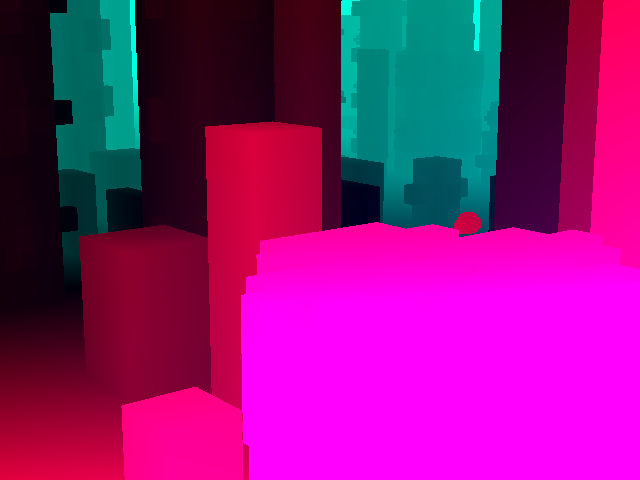
\includegraphics[width=0.48 \columnwidth] {urban2_truth.png} 

\caption{Results for the ``Urban2" test image.  Top left: one of the two input frames.  Top right: optical flow using the HS algorithm, with average error 6.95.  Bottom left: optical flow using multi-resolution HS, with average error 1.79.  Bottom right: ground truth.  The flow magnitude is too large for HS to handle correctly.  Using multi-resolution optimization, we can locate large flows with much better accuracy.}
\label{fig:urban2}
\end{figure}

\section{Solving Optical Flow with a Charbonnier Penalty}

We would now like to use the Charbonnier penalty in our flow objective function.  With the Charbonnier penalty on flow smoothness, our objective function becomes
\begin{multline} \label{eq:objectivec}
e = \int \int_{img} (I_x \cdot X + I_y \cdot Y + I_t)^2 + \\
\lambda \sqrt{X_x^2 + X_y^2 + Y_x^2 + Y_y^2 + \epsilon} \; dA 
\end{multline}

To derive a minimum for this function, it's best to express it in discrete form:
\begin{multline} \label{eq:objectivecDiscrete}
e = \sum_{i,j} (I_x(i, j) X(i, j) + I_y(i, j) Y(i, j) + I_t(i, j))^2 \\
+ \lambda \sqrt{
\begin{array}{c}
(X(i, j) - X(i-1, j))^2 \\
+ (X(i,j) - X(i,j-1))^2 \\
+ (Y(i,j) - Y(i-1, j))^2 \\
+ (Y(i,j) - Y(i,j-1))^2 + \epsilon
\end{array}
}
\end{multline}
To save space, let us name the error and regularization terms:
\begin{multline} \label{eq:errorTerm}
Err(i, j) = I_x(i, j) X(i, j) \\
+ I_y(i, j) Y(i, j) + I_t(i, j)
\end{multline}
\begin{equation} \label{eq:regTerm}
Reg(i,j) = (X(i,j) - X(i-1,j))^2 + ...
\end{equation}

Now, our objective function becomes:
\begin{equation} \label{eq:shortobjcdis}
e = \sum_{i,j} Err(i,j)^2 + \lambda \sqrt{Reg(i,j) + \epsilon }
\end{equation}
To minimize the objective function in Eq. \ref{eq:shortobjcdis}, we take the straightforward approach: calculate a derivative with respect to $X(i, j)$.  By setting each derivative equal to $0$, we hope to get an approximation for the $X$ and $Y$ that minimize $e$.
\begin{equation}
\begin{aligned}
&\frac{\partial e}{\partial X(i, j)} = \frac{\partial Err(i,j)}{\partial X(i, j)} \cdot 2 Err(i, j) \\
&+ \lambda \frac{\partial Reg(i,j)}{\partial X(i, j)} \cdot \frac{1}{2} (Reg(i, j) + \epsilon)^{-0.5}  \\
&+ \lambda \frac{\partial Reg(i+1,j)}{\partial X(i, j)} \cdot \frac{1}{2} (Reg(i+1, j) + \epsilon)^{-0.5}  \\
&+ \lambda \frac{\partial Reg(i,j+1)}{\partial X(i, j)} \cdot \frac{1}{2} (Reg(i, j+1) + \epsilon)^{-0.5}
\end{aligned}
\label{eq:dedx}
\end{equation}
Notice that only one error term depends on $X(i, j)$, but three separate regularization terms depend on $X(i, j)$.

Now, we want to evaluate the individual partial derivatives:
\begin{equation} \label{eq:derrdx}
\frac{\partial Err(i,j)}{\partial X(i, j)} = I_x(i, j)
\end{equation}
\begin{equation} \label{eq:dreg1dx}
\begin{aligned}
&\frac{\partial Reg(i,j)}{\partial X(i, j)} \\
&= 2(X(i, j) - X(i-1, j)) + 2(X(i, j) - X(i, j-1)) \\
&= 2X(i,j) - X(i-1, j) - X(i,j-1)
\end{aligned}
\end{equation}
\begin{equation} \label{eq:dreg2dx}
\frac{\partial Reg(i+1,j)}{\partial X(i, j)} = -2(X(i+1,j) - X(i,j))
\end{equation}
\begin{equation} \label{eq:dreg3dx}
\frac{\partial Reg(i,j+1)}{\partial X(i, j)} = -2(X(i,j+1) - X(i,j))
\end{equation}

Finally, we assume that nearby regularization terms are approximately equal: $Reg(i, j) \approx Reg(i+1,j) \approx Reg(i,j+1)$.  We can now simplify the derivative in Eq. \ref{eq:dedx}, resulting in a very familiar form:
\begin{equation} \label{eq:leastsq}
\begin{aligned}
0 = \frac{\partial e}{\partial X(i, j)} &= 2I_x(i, j) Err(i, j)  \\
+\lambda(&\\
&4X(i, j) - X(i+1,j) \\
&- X(i-1,j) - X(i,j+1) - X(i,j-1) \\
&)\cdot (Reg(i, j) + \epsilon) ^{-0.5}
\end{aligned}
\end{equation}

Note that the terms in parentheses are exactly $(D_{xx} + D_{yy}) X$, the sum of the second derivatives of $X$ evaluated at $(i, j)$.  Also, $(Reg(i, j) + \epsilon)^{-0.5}$ is the only term not linear in $X$.  Therefore, we can use iteratively-reweighted least squares to solve this equation.  In this formulation,
\begin{equation} \label{eq:weights}
W(i,j) = (Reg(i,j) + \epsilon)^{-0.5}
\end{equation}
will be the weights.  We will repeatedly solve for $X$ and $Y$, recompute the weights, then re-solve for $X$ and $Y$.  Our derivative constraint in Eq. \ref{eq:leastsq} now becomes
\begin{equation} \label{eq:leastsqx}
\begin{aligned}
2I_x (I_x X + I_y Y + I_t) \\
 -\lambda(D_{xx} + D_{yy}) X \cdot W = 0
\end{aligned}
\end{equation}

There exists an analogous equation obtained by taking a derivative with respect to $Y$:
\begin{equation} \label{eq:leastsqy}
\begin{aligned}
2I_y (I_x X + I_y Y + I_t) \\
 -\lambda(D_{xx} + D_{yy}) Y \cdot W = 0
\end{aligned}
\end{equation} 
We can combine all $2wh$ equations into block matrix form, to obtain an equation very similar to Eq. \ref{eq:eulerBlock}:
\begin{multline} \label{eq:leastsqBlock}
\left[ \begin{array}{cc}
I_x^2 - \lambda W (D_x^2 + D_y^2) & I_x I_y\\
I_x I_y & I_y^2 - \lambda W (D_x^2 + D_y^2) \\
\end{array} \right]
\left[\begin{array}{c}
X \\
Y
\end{array} \right] \\
=-\left[ \begin{array}{c}
I_x I_t \\
I_y I_t
\end{array} \right]
\end{multline}
Once again, an aside on notation is necessary here.  The term $\lambda W (D_x^2 + D_y^2) X$ refers to the following steps: (1) evaluate the sum of the second derivatives at $X$ using the Laplacian filter.  Put these values in a column vector of length $wh$, because $X$ is a column vector and $D_x$ is an operator.  (2) Multiply the column vector by the diagonal matrix $\lambda W$.

To solve for the flow using this equation, we use the same technique developed for solving the original HS equation, with one addition: we recalculate $W$ at every turn.  $W$ is recalculated using the values of $X$ and $Y$ found in the last iteration, according to Eq. \ref{eq:weights}.
{\small
\bibliographystyle{ieee}
\bibliography{egbib}
}

\end{document}
